\section{A Toy Model}
\label{s:toymodel}

\subsection{Formulation}
\label{s:toy_formalism}
\markboth{\MakeUppercase{\thechapter. Toy Models }}{\thechapter. Toy Models}

\paragraph{}To get the feel of Compressed Sensing, we applied its framework on various toy models. 
One such model is spike train model in which $A$ matrix or sensing matrix of order $M \times N$ is 
random Gaussian matrix with normalized i.i.d entries. We constructed hypothetical example with known $M=40$ 
random measurements ($b$ vector) for a particular $40 \times 100$ $A$ matrix and it is also known that $x$ 
vector which we have to reconstruct, has four spikes. Figure (\ref{Figorgvect} is an plot of original vector
in which $X$-axis denotes the component number and $Y$ axis represents values at each components. Indeed  
$x$ is sparse as most of its components are either zero or approximately equal to zero. We had also added 
normally distributed Gaussian noise in the measurement vector as in real scenario every measurements comes with the noise.


\subsection{Tools used}
\label{s:toy_tools}
\paragraph{}Next step was to apply compressed sensing or $\ell_1$ minimization algorithms to this problem, we used MATLAB 
as a tool for this analysis and CVX, which is matlab program for disciplined convex programming, is used to solve \ref{1.6}
formulated for this problem. ( for more information refer CVX user Guide ).

\subsection{Results and Discussion}
\label{s:toy_results}
\paragraph{}Figure \ref{Figorgvect} shows plot of original vector with X-axis as component number and 
Y-axis as corresponding value at each components. Figure shows that plotted vector is sparse and has 
only four significant values or spikes. 
\paragraph{}Figure \ref{Figrecvect} shows plot of reconstructed vector (shown with dotted red line) and
original vector (dotted blue line). With small variation reconstructed vector overlaps the original
vector.
\paragraph{}CVX internally use Interior point methods (\cite{karmarkar}) for solving equation (\ref{1.6}) for the given problem.
This basic linear programming method has no performance issues while dealing with problems of such small scale
but suffer for poor convergence rate otherwise. For this toy problem, interior point algorithm or CVX converges in 
127 iterations. Further, CVX does not require any penalty parameter for minimization process. 

\begin{figure}[!htbp]
  \begin{center}
      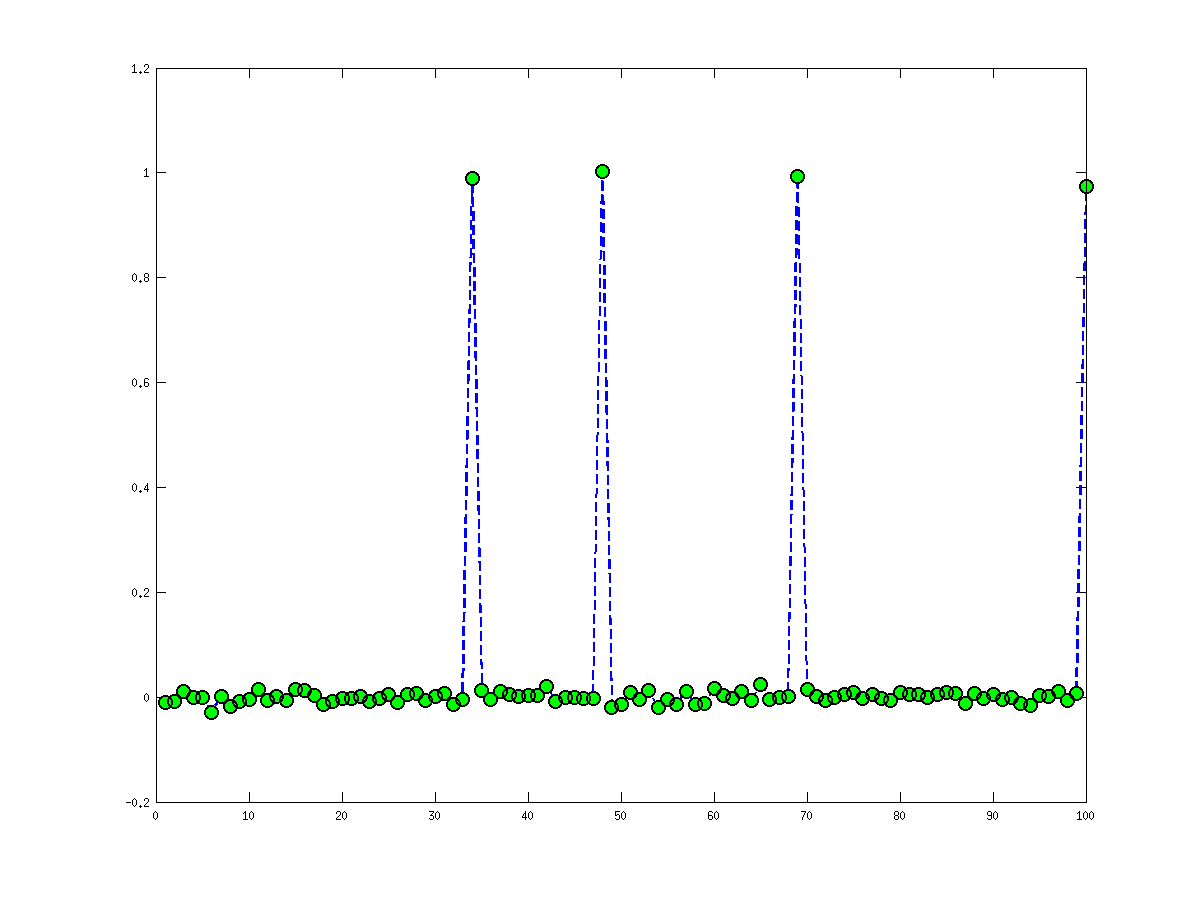
\includegraphics[width=6.1in,height=4in]{figures/orgvect}
    \caption{Original Vector}
    \label{Figorgvect}
  \end{center}

\end{figure}
\begin{figure}[!htbp]
  \begin{center}
      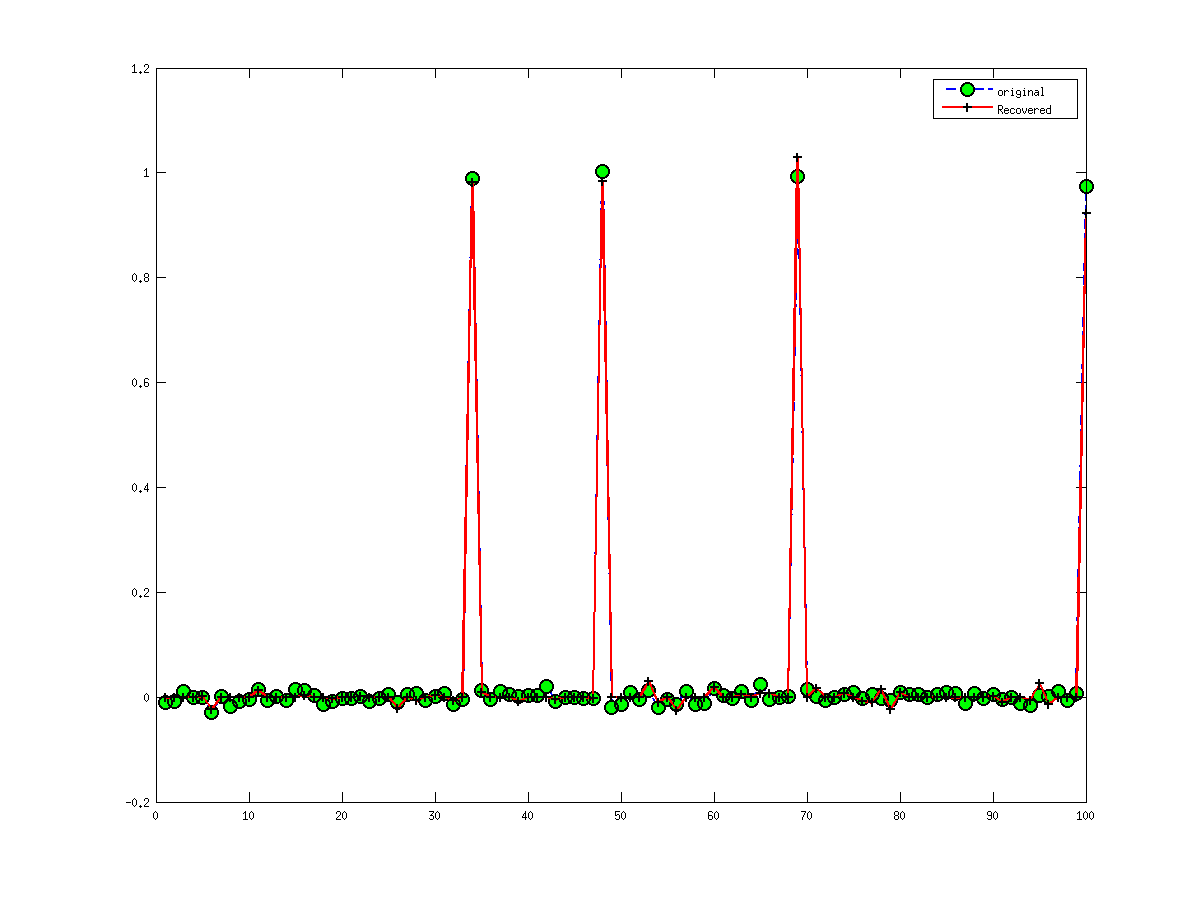
\includegraphics[width=6.1in,height=4in]{figures/recvect}
    \caption{Reconstructed Vector}
    \label{Figrecvect}
  \end{center}
\end{figure}
